% !TeX program = pdflatex
% Build: latexmk -pdf -interaction=nonstopmode -halt-on-error ISMS_Build_Buy_Hybrid_Decision_Framework.tex
% Edition: 17 October 2026 | Illustrative financials, not vendor quotations.
\documentclass[10pt,letterpaper]{article}
\usepackage[T1]{fontenc}
\usepackage[utf8]{inputenc}
\usepackage{lmodern}
\usepackage[letterpaper,left=0.82in,right=0.82in,top=0.85in,bottom=0.80in,headheight=15pt]{geometry}
\usepackage{microtype}
\usepackage[table]{xcolor}
\usepackage{amsmath,amssymb}
\usepackage{booktabs,tabularx,longtable,array,multirow}
\usepackage{pdflscape}
\usepackage{graphicx}
\usepackage{tikz}
\usetikzlibrary{arrows.meta,positioning,fit,backgrounds,calc,shapes.geometric}
\usepackage{tcolorbox}
\tcbuselibrary{breakable,skins}
\usepackage{enumitem}
\usepackage{fancyhdr,lastpage}
\usepackage{titlesec}
\usepackage{hyperref}
\usepackage{cleveref}
\usepackage{listings}
\usepackage{float}
\usepackage{caption}
\usepackage{needspace}
\usepackage{multicol}
\usepackage{pgfplots}
\pgfplotsset{compat=1.18}
\definecolor{navy}{HTML}{102A43}
\definecolor{ink}{HTML}{23364A}
\definecolor{teal}{HTML}{087F8C}
\definecolor{pale}{HTML}{E9F4F5}
\definecolor{bluepale}{HTML}{EDF3F8}
\definecolor{muted}{HTML}{5B6C7C}
\definecolor{line}{HTML}{D6E0E8}
\definecolor{gold}{HTML}{B7791F}
\definecolor{warm}{HTML}{FFF6E6}
\definecolor{paper}{HTML}{F8FAFC}
\color{ink}
\hypersetup{colorlinks=true,linkcolor=navy,urlcolor=teal,citecolor=navy,pdftitle={Build vs Buy vs Hybrid: ISMS Engineering and Software Acquisition Decision Framework},pdfauthor={Engineering Reference},pdfsubject={ISO/IEC 27001 ISMS acquisition, architecture, evaluation, TCO, roadmap}}
\urlstyle{same}
\setlength{\parindent}{0pt}
\setlength{\parskip}{5.5pt}
\setlist[itemize]{leftmargin=1.45em,topsep=2pt,itemsep=2pt,parsep=0pt}
\setlist[enumerate]{leftmargin=1.5em,topsep=2pt,itemsep=3pt,parsep=0pt}
\renewcommand{\arraystretch}{1.17}
\newcolumntype{Y}{>{\raggedright\arraybackslash}X}
\newcolumntype{L}[1]{>{\raggedright\arraybackslash}p{#1}}
\newcolumntype{R}[1]{>{\raggedleft\arraybackslash}p{#1}}
\titleformat{\section}{\color{navy}\Large\bfseries}{\thesection}{0.65em}{}[\vspace{-0.3em}\color{line}\titlerule]
\titleformat{\subsection}{\color{navy}\large\bfseries}{\thesubsection}{0.6em}{}
\titleformat{\subsubsection}{\color{teal}\normalsize\bfseries}{\thesubsubsection}{0.6em}{}
\titlespacing*{\section}{0pt}{18pt}{10pt}
\titlespacing*{\subsection}{0pt}{13pt}{5pt}
\pagestyle{fancy}
\fancyhf{}
\fancyhead[L]{\footnotesize\sffamily\color{muted} ISMS ENGINEERING / ACQUISITION}
\fancyhead[R]{\footnotesize\sffamily\color{muted} REFERENCE EDITION \;|\; 2026-10-17}
\fancyfoot[L]{\footnotesize\sffamily\color{muted} Internal decision-support template}
\fancyfoot[R]{\footnotesize\sffamily\color{muted} \thepage\ / \pageref{LastPage}}
\renewcommand{\headrulewidth}{0.35pt}
\renewcommand{\footrulewidth}{0pt}
\newtcolorbox{noteBox}[1][]{enhanced,breakable,colback=bluepale,colframe=line,boxrule=0.5pt,arc=1mm,left=8pt,right=8pt,top=6pt,bottom=6pt,#1}
\newtcolorbox{decisionBox}[1][]{enhanced,breakable,colback=pale,colframe=teal,boxrule=0.65pt,arc=1mm,left=9pt,right=9pt,top=7pt,bottom=7pt,#1}
\newtcolorbox{cautionBox}[1][]{enhanced,breakable,colback=warm,colframe=gold,boxrule=0.65pt,arc=1mm,left=9pt,right=9pt,top=7pt,bottom=7pt,#1}
\newcommand{\tagreq}{\textsf{REQ}}
\newcommand{\tagguide}{\textsf{GUIDANCE}}
\newcommand{\tagmodel}{\textsf{ILLUSTRATIVE}}
\newcommand{\USD}[1]{\$#1}
\newcommand{\tinylabel}[1]{\textsf{\footnotesize\color{teal}\MakeUppercase{#1}}}
\newcommand{\figsource}[1]{\par\vspace{-4pt}{\footnotesize\color{muted}\textit{#1}}}
\newcommand{\refweb}[2]{\href{#1}{#2}}
\lstdefinestyle{readable}{basicstyle=\ttfamily\footnotesize,breaklines=true,columns=fullflexible,frame=single,rulecolor=\color{line},backgroundcolor=\color{paper},showstringspaces=false,keywordstyle=\color{teal}\bfseries,commentstyle=\color{muted},xleftmargin=4pt,xrightmargin=4pt}
\lstset{style=readable}
\begin{document}
\thispagestyle{empty}
\begin{tikzpicture}[remember picture,overlay]
  \fill[navy] (current page.north west) rectangle ([yshift=-2.30in]current page.north east);
  \fill[teal] ([yshift=-2.28in]current page.north west) rectangle ([yshift=-2.38in]current page.north east);
  \draw[white!24,line width=0.7pt] ([xshift=-2.6in,yshift=-0.25in]current page.north east) circle (2.1in);
  \draw[white!25,line width=0.7pt] ([xshift=-2.6in,yshift=-0.25in]current page.north east) circle (1.60in);
  \draw[white!26,line width=0.7pt] ([xshift=-2.6in,yshift=-0.25in]current page.north east) circle (1.05in);
\end{tikzpicture}
\vspace*{0.42in}
{\sffamily\color{white}\bfseries\Large SECURITY ARCHITECTURE / ENTERPRISE PROCUREMENT}\par\vspace{0.22in}
{\sffamily\color{white}\fontsize{29}{35}\selectfont\bfseries BUILD \;/\; BUY \;/\; HYBRID}\par\vspace{0.08in}
{\sffamily\color{white}\Large Information Security Management System}\par
\vspace*{1.15in}
{\sffamily\fontsize{23}{28}\selectfont\bfseries Engineering and Software\\Acquisition Decision Framework}\par\vspace{0.25in}
{\Large Architecture models \quad Requirements \quad Economics\\ Procurement scorecards \quad Implementation roadmap}\par\vspace{0.42in}
\begin{tcolorbox}[enhanced,colback=paper,colframe=line,arc=1mm,boxrule=0.6pt]
\tinylabel{Purpose}\par
A repeatable method to select, architect, procure, govern, and operate ISMS-enabling software while preserving independent responsibility for information-security management and ISO/IEC 27001 conformity.\par
\smallskip

\begin{tabularx}{\linewidth}{@{}L{1.17in}Y@{}}
\textbf{Baseline} & ISO/IEC 27001:2022, Amendment 1:2024; related ISO guidance and NIST risk-management resources.\\
\textbf{Audience} & CISO, GRC, enterprise architecture, engineering, procurement, finance, privacy, legal, and internal audit.\\
\textbf{Decision} & Build an internal platform; procure commercial software; or deploy a governed hybrid with interoperable automation.\\
\textbf{Status} & Reusable evaluation framework; not legal advice, vendor certification, or a substitute for licensed standards.\\
\end{tabularx}
\end{tcolorbox}
\vfill
{\sffamily\color{navy}\bfseries Version 1.0 \quad | \quad 17 October 2026}\par
{\sffamily\color{muted} Includes fully worked illustrative 5-year TCO and decision scoring. All monetary assumptions require organization-specific validation.}
\clearpage
\begin{noteBox}
\textbf{Reading protocol.} Labels have deliberately different meanings: \textbf{Standard topic} is a paraphrase of the published management-system requirement; \textbf{Engineering recommendation} is a proposed control or software implementation; \textbf{Illustrative} marks unverified sample inputs or scenario outputs. Obtain the licensed standards and jurisdiction-specific advice before making a conformity claim.
\end{noteBox}
\tableofcontents
\clearpage

\section{Executive decision brief}
\subsection{Decision to be made}
Select the \emph{software and operating architecture supporting an ISMS}, not whether the organization will operate an ISMS. ISO/IEC 27001:2022 defines requirements for the management system itself; accountability, leadership, risk ownership, evidence quality, internal audit, and continual improvement do not transfer to a software supplier \cite{iso27001,iso27002}. A commercial platform can accelerate administration, but neither platform purchase nor policy-template population establishes conformity or guarantees certification.

\begin{decisionBox}
\textbf{Default hypothesis, pending validation:} Shortlist a \textbf{hybrid} architecture for a medium-to-large, integration-heavy enterprise: a managed system of record for governance and audit workflows, supported by internally governed collectors and evidence-validation services. Choose \textbf{buy} when standardization and speed dominate; choose \textbf{build} only when specialized workflows, strict data boundaries, proven internal capabilities, and defensible lifecycle economics outweigh delivery risk.
\end{decisionBox}

\subsection{Executive one-page scorecard}

\begin{tabularx}{\linewidth}{@{}L{1.08in}YYY@{}}
\toprule
\textbf{Criterion} & \textbf{Build} & \textbf{Buy} & \textbf{Hybrid}\\\midrule
Primary strength & Differentiated workflow and full source control & Fast adoption and managed feature delivery & Standard governance with tailored integrations\\
Primary weakness & Engineering burden, continuity risk & Dependency, portability and contract limits & Split ownership and integration complexity\\
Best when & Unique requirements are stable and critical & Requirements match proven product capabilities & Enterprise-specific systems must feed standardized GRC\\
Failure signal & Delivery backlog exceeds risk-reduction benefits & Workflow/data exit restrictions block objectives & Connectors lack traceable ownership or quality\\
\bottomrule
\end{tabularx}

\subsection{Non-negotiable exit criteria}
\begin{enumerate}
\item Approved scope, interested parties, risk criteria, owner assignments and decision authority exist independently of platform choice.
\item All material data flows, regulated-data handling, processor responsibilities, retention obligations and location constraints have been reviewed.
\item A working end-to-end sample demonstrates \textbf{source event $\rightarrow$ validated evidence $\rightarrow$ control evaluation $\rightarrow$ reviewer sign-off $\rightarrow$ auditor export}.
\item Finance signs off on a comparable five-year TCO, including common costs, excluded costs, risk contingencies and sensitivity analyses.
\item Vendor contract or internal architecture provides credible recovery, export, exit, incident notification and continuity provisions.
\end{enumerate}

\subsection{What the illustrative calculations indicate}

\begin{tabularx}{\linewidth}{@{}YYYY@{}}
\toprule
\textbf{5-year example, USD thousands} & \textbf{Build} & \textbf{Buy} & \textbf{Hybrid}\\\midrule
Year-zero implementation & 260 & 95 & 155\\
Year-one option-specific operating cost & 160 & 150 & 135\\
Annual cost escalation & 4\% & 5\% & 4\%\\
Five-year nominal TCO & 1,126.61 & 923.84 & \textbf{886.20}\\
Five-year NPV at 10\% & 912.14 & 717.59 & \textbf{705.25}\\
Weighted capability score (0--100) & 73 & 76 & \textbf{85}\\
\bottomrule
\end{tabularx}
\figsource{Illustrative, invented planning inputs; no vendor-specific pricing. Nominal and NPV values are calculated from the exact model in Section~\ref{sec:finance}. Scores are subjective demonstration inputs, not measured benchmarks.}

\section{Governance baseline and scope}
\subsection{Source hierarchy and standards status}

\begin{tabularx}{\linewidth}{@{}L{1.43in}L{1.12in}Y@{}}
\toprule
\textbf{Reference} & \textbf{Status in this framework} & \textbf{Use}\\\midrule
ISO/IEC 27001:2022, Amd 1:2024 & Conformity baseline & ISMS requirements, risk-treatment process, leadership, performance evaluation, improvement; explicitly consider climate-change relevance in organizational context \cite{iso27001,iso27001am}.\\
ISO/IEC 27002:2022 & Informative guidance & Implementation guidance for information-security controls, not an independent certification checklist \cite{iso27002}.\\
ISO/IEC 27005:2022 & Informative guidance & Information-security risk assessment and treatment methods \cite{iso27005}.\\
ISO 19011:2026 & Informative guidance & Management-system audit-program and auditor-practice design \cite{iso19011}.\\
NIST CSF 2.0 & Complementary framework & Outcome-based cyber-risk communication, especially the Govern function \cite{nistcsf}.\\
NIST SP 800-161 Rev. 1; SP 1326 & Complementary guidance & Supplier risk and due diligence for ICT acquisitions \cite{nist161,nist1326}.\\
\bottomrule
\end{tabularx}

\subsection{What is in scope}
The evaluation covers risk and treatment registers; Statement of Applicability (SoA); controls inventory; policies and exceptions; asset/service ownership; control monitoring; evidence collection and preservation; internal-audit support; management review; findings and corrective actions; third-party risk; identity and access; reporting; integrations; and vendor operations. Excluded by default are replacing endpoint security, SIEM, IAM, vulnerability scanners, ticketing, or full enterprise resource planning. The acquired platform \emph{coordinates} those systems rather than automatically replacing them.

\subsection{ISO/IEC 27001 management-system traceability}
\small

\begin{longtable}{@{}L{0.59in}L{1.52in}L{2.13in}L{2.12in}@{}}
\toprule
\textbf{Clause} & \textbf{Standard topic (paraphrase)} & \textbf{Recommended capability / retained responsibility} & \textbf{Typical evidence / validation}\\\midrule\endhead
4 & Organizational context, stakeholders, scope and ISMS & Scope register, context review, interested-party register; context owners remain accountable & Approved scope, context changes, stakeholder review, climate relevance determination\\
5 & Leadership, policy and roles & Policy approval, delegation, roles and responsibilities, documented management commitment & Board/executive decisions, policy sign-off, authority matrix\\
6 & Risk-based planning and objectives & Defined assessment/treatment method; risk register; SoA; measurable objectives & Risks and approvals, treatment plan, SoA rationale, objectives and plans\\
7 & Resources, competence, awareness, communication, documentation & Document lifecycle, training and competence records, controlled access & Version history, attendance, publishing approvals, record retention\\
8 & Operational planning, risk assessment and treatment & Assessment cadence, triggered reassessment, control operations & Results of risk reviews, treatment decisions, operational records\\
9 & Monitoring, measurement, analysis, audit, management review & Measure register, independent internal-audit workflow, executive-review pack & Metrics, audit program and outputs, review decisions\\
10 & Nonconformity, corrective action, continual improvement & Corrective action workflow with verification and closed-loop learning & Root-cause, action plan, effectiveness check, closure approvals\\
Annex A & Reference controls for control comparison & Risk-derived selection and exclusion rationale in SoA; mapping is not ``select all'' & SoA decisions, implementation status, evidence and reviews\\
\bottomrule
\end{longtable}
\normalsize
\begin{cautionBox}
\textbf{Conformity boundary.} Annex A provides a reference set against which selected controls are checked for completeness; it does not eliminate risk-based selection, and the SoA is not equivalent to a vendor's ``percent controls enabled'' dashboard. The 2022 control set has 93 controls organized into organizational (37), people (8), physical (14), and technological (34) themes \cite{iso27002}. Do not claim an automated ``ISO score'' is a certification determination.
\end{cautionBox}

\subsection{Three distinct assurances}
\begin{enumerate}
\item \textbf{Design adequacy:} Are risks, policies, control objectives, methods, owners, and authority suitable for the business?
\item \textbf{Operating effectiveness:} Do actual activities occur on schedule and produce relevant, reliable evidence over the period tested?
\item \textbf{Independent assurance:} Can internal auditors and, if chosen, external certification bodies independently evaluate the ISMS, including excluded controls and exceptions?
\end{enumerate}

\section{Business case, boundary conditions and option taxonomy}
\subsection{Business-case intake}
Record the following before contacting suppliers: organization size, ISMS scope, entities/locations, target certification or customer-assurance dates, required frameworks, asset/application inventory coverage, current systems of record, security and privacy classifications, evidence volume, integration count, audit cycles, support model, budget, required data residency, and internal engineering capacity. Mark absent or unverifiable inputs \textbf{unknown}, never zero.

\subsection{Decision drivers}

\begin{tabularx}{\linewidth}{@{}L{1.28in}YYY@{}}
\toprule
\textbf{Driver} & \textbf{Build advantage} & \textbf{Buy advantage} & \textbf{Hybrid advantage}\\\midrule
Regulatory specificity & Custom logic if mature & Standardized reporting if supported & Central governance plus specialized validation\\
Time-to-first-audit & Risk of delay & Packaged workflows & Phased control coverage\\
Integration breadth & Engineering can address all & Depends on connectors & Custom adapters preserve core workflows\\
Data ownership & Full control of code/data paths & Contractual & Segregated raw evidence and governance data\\
Operating resilience & Internal SRE ownership & SLA/vendor operation & Platform SLA and internal evidence pipeline SLOs\\
Change velocity & Internal product roadmap & Supplier release train & Adaptable integration perimeter\\
\bottomrule
\end{tabularx}

\subsection{Define mutually comparable alternatives}
\textbf{B1 --- Internal build.} Owned application, risk/control data services, workflow engine, evidence connectors, secure file store, reporting, audit exports, operations and documentation. Existing commodity cloud, database, IdP and CI services may still be purchased; ``build'' is not zero third-party cost.

\textbf{P1 --- Commercial buy.} Single ISMS/GRC SaaS or licensed platform, configured for the operating model. Product-native integrations provide evidence; special integrations are optional and separately estimated. The buyer retains risk decisions, validation and audits.

\textbf{H1 --- Governed hybrid.} Commercial GRC/ISMS system of record + internally owned integration/evidence service + enterprise object storage/data retention + ticketing and policy repositories. Draw contracts, data classification and export boundaries first; avoid dual masters for risk, control or evidence lifecycle state.

\subsection{Hard gates before weighted scoring}
\small

\begin{longtable}{@{}L{0.66in}L{2.25in}L{3.59in}@{}}
\toprule
\textbf{Gate} & \textbf{Pass criterion} & \textbf{Required demonstration}\\\midrule\endhead
G-01 & Lawful data handling and defined residency & Data-flow diagram; processor/subprocessor list; retention; access controls; legal review\\
G-02 & Exportability and exit viability & Machine-readable risk, SoA, controls, evidence metadata, audit events; binary attachments; documented IDs\\
G-03 & Security baseline & SSO/MFA, least privilege, audit records, encrypted transport/storage, incident response and secure SDLC\\
G-04 & Evidence integrity & Traceable source, collector version, timestamp, transformation, approving reviewer and tamper detection\\
G-05 & Workflow viability & Risk $\rightarrow$ treatment $\rightarrow$ SoA $\rightarrow$ control $\rightarrow$ evidence $\rightarrow$ finding\\
G-06 & Delivery capacity & Funded named owners, feasible staffing, support and disaster recovery commitment\\
G-07 & Contract / procurement & Acceptable liability, breach notice, subprocessor changes, deletion, renewal and termination terms\\
G-08 & Audit independence & Internal-audit role separation, read-only auditor access, export and documented findings process\\
\bottomrule
\end{longtable}
\normalsize
\textbf{Rule:} An alternative failing a non-waivable gate is ineligible regardless of weighted score. Where law or regulatory commitments require an exception, record a formal accountable decision and avoid marketing it as compliant.

\section{Capability and requirements engineering}
\subsection{Requirements conventions and verification}
IDs are stable for traceability. Priority \textbf{M} = must-have at production acceptance; \textbf{S} = should-have by planned phase; \textbf{C} = could-have. Acceptance must be demonstrated against scoped real or sanitized datasets, not slides or an unconfigured sales environment.

\small

\begin{longtable}{@{}L{0.58in}L{0.36in}L{2.55in}L{2.87in}@{}}
\toprule
\textbf{ID} & \textbf{Pri.} & \textbf{Functional requirement} & \textbf{Acceptance demonstration}\\\midrule\endfirsthead
\toprule\textbf{ID} & \textbf{Pri.} & \textbf{Functional requirement} & \textbf{Acceptance demonstration}\\\midrule\endhead
FR-01 & M & Versioned ISMS scope and entities & Approve, change and retrieve scope with history\\
FR-02 & M & Interested-party, obligations and context registry & Link requirement to owner and review decision\\
FR-03 & M & Risk assessment method and register & Reproducible scoring with controlled criteria\\
FR-04 & M & Risk ownership, acceptance and treatment & Role-gated acceptance with expiry/reassessment\\
FR-05 & M & Statement of Applicability & Map controls, inclusion/exclusion rationale, status, version and approver\\
FR-06 & M & Control catalog, objectives and owners & Map framework IDs to tailored control implementation\\
FR-07 & M & Evidence objects and provenance & Retrieve immutable metadata and original payload by ID\\
FR-08 & M & Evidence/control review and exceptions & Reviewer can approve, reject or document exception\\
FR-09 & M & Policy/standard/record lifecycle & Draft, review, publish, supersede and archive\\
FR-10 & M & Internal audit planning and findings & Plan, independence checks, sampled evidence, report\\
FR-11 & M & Corrective actions and effectiveness & Action assignment, root cause, closure and verification\\
FR-12 & M & Management review package & Generate reviewed inputs, decisions and assigned actions\\
FR-13 & M & Role-based access + SSO/MFA & Assert separation-of-duty test cases\\
FR-14 & M & Search and certified-scope export & Export data, links, audit trails and attachments\\
FR-15 & M & System and user audit trails & Tamper-evident identity/time/action/context logging\\
FR-16 & S & Scheduled evidence ingestion & Source mapping, retries, freshness and reconciliation\\
FR-17 & S & Metrics, trend and overdue escalation & Drill down from KPI to record and source event\\
FR-18 & S & Third-party risk assessment & Supplier owners, due-diligence outcome and residual risk\\
FR-19 & S & Jira/ServiceNow and repository integration & Stable object IDs, webhook replay and reconciliation\\
FR-20 & S & Multi-framework control mapping & Versioned, reviewable mapping with non-equivalence caveat\\
FR-21 & S & Asset/service inventory association & Control/test mapped to system and accountable owner\\
FR-22 & S & Policy acknowledgement and awareness & Evidence of assignment, completion and exceptions\\
FR-23 & C & Continuous control testing & Store test code/version and human adjudication decision\\
FR-24 & C & API-based automated evidence package & Export signed manifest + normalized bundle\\
\bottomrule
\end{longtable}
\normalsize
\subsection{Nonfunctional requirements}
\small

\begin{longtable}{@{}L{0.60in}L{0.37in}L{2.45in}L{2.94in}@{}}
\toprule
\textbf{ID} & \textbf{Pri.} & \textbf{Requirement / target (proposed)} & \textbf{Evidence of conformance}\\\midrule\endhead
NFR-01 & M & No unauthorized access across tenants and roles & Adversarial RBAC/ABAC test and tenancy design review\\
NFR-02 & M & IdP SSO, enforced MFA and timely deprovisioning & Provision, disable, revoke tokens, verify logs\\
NFR-03 & M & Encryption in transit and at rest; key ownership specified & TLS verification, key lifecycle and architecture review\\
NFR-04 & M & Defined RPO $\leq 24$ h and RTO $\leq 8$ h (\emph{example}) & Restore rehearsal and signed recovery report\\
NFR-05 & M & Recovery and export without proprietary client & Portable extraction on representative scope\\
NFR-06 & M & Append-only event trail, protected against alteration & Security review, retention and integrity check\\
NFR-07 & M & Data retention/deletion by class and legal hold & Demonstrate expiry, purge and hold precedence\\
NFR-08 & M & Supplier incident notification and support path & Executed contract, tabletop and escalation drill\\
NFR-09 & S & Automated connector retry/idempotency & Fault injection and repeated ingestion test\\
NFR-10 & S & Evidence freshness SLO by control criticality & Detect overdue collection and trigger escalation\\
NFR-11 & S & 99.9\% monthly availability objective (\emph{example}) & Measured SLI exclusions and SLA credits reviewed\\
NFR-12 & S & API limits, throughput and pagination specified & Load test with expected growth and burst requests\\
NFR-13 & S & Infrastructure-as-code and environment promotion & Reproducible deployment with controlled approvals\\
NFR-14 & S & Region, subprocessor and transfer transparency & Supplier data map and transfer assessment\\
NFR-15 & S & WCAG-relevant accessibility requirements & Accessibility acceptance testing\\
NFR-16 & C & Threat detection and anomaly alert integration & SecOps correlation and incident drill\\
\bottomrule
\end{longtable}
\normalsize
\subsection{Traceability ledger --- minimum joins}
\begin{noteBox}
\texttt{BusinessObjective $\rightarrow$ Risk $\rightarrow$ TreatmentDecision $\rightarrow$ SoAEntry $\rightarrow$ ControlImplementation $\rightarrow$ ControlTest $\rightarrow$ EvidenceObject $\rightarrow$ Finding/Exception $\rightarrow$ CorrectiveAction $\rightarrow$ ClosureVerification}. Each edge needs a stable identifier, ownership, version, timestamp and reason for change. Framework mappings are many-to-many, versioned, and manually approved when not exact equivalence.
\end{noteBox}

\section{Architecture models and integration design}
\subsection{Context architecture: responsibility boundaries}
\begin{figure}[H]
\centering
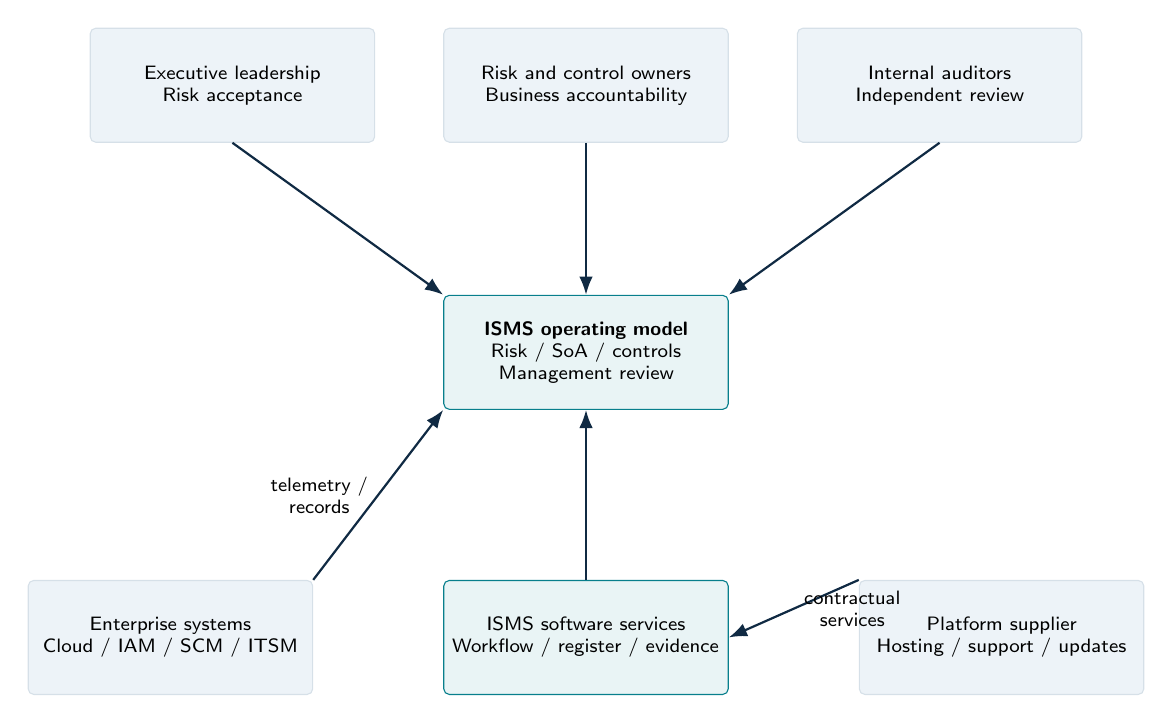
\begin{tikzpicture}[font=\sffamily\scriptsize,box/.style={draw=line,fill=bluepale,rounded corners=2pt,align=center,text width=1.33in,minimum height=0.57in},critical/.style={box,draw=teal,fill=pale},arr/.style={-Latex,thick,draw=navy},node distance=0.51in and 0.34in]
\node[box] (board) {Executive leadership\\ Risk acceptance};
\node[box,right=of board] (owners) {Risk and control owners\\ Business accountability};
\node[box,right=of owners] (audit) {Internal auditors\\ Independent review};
\node[critical,below=0.76in of owners] (core) {\textbf{ISMS operating model}\\ Risk / SoA / controls\\ Management review};
\node[box,below left=0.85in and 0.65in of core] (source) {Enterprise systems\\ Cloud / IAM / SCM / ITSM};
\node[critical,below=0.85in of core] (platform) {ISMS software services\\ Workflow / register / evidence};
\node[box,below right=0.85in and 0.65in of core] (supplier) {Platform supplier\\ Hosting / support / updates};
\draw[arr] (board.south) -- (core.north west);
\draw[arr] (owners.south) -- (core.north);
\draw[arr] (audit.south) -- (core.north east);
\draw[arr] (source.north east) -- node[left,align=center]{telemetry /\\records} (core.south west);
\draw[arr] (platform.north) -- (core.south);
\draw[arr] (supplier.north west) -- node[right,align=center]{contractual\\services} (platform.east);
\end{tikzpicture}
\caption{ISMS accountability remains organizational; software is an enabling subsystem.}
\end{figure}

\subsection{Hybrid reference architecture: logical components}
\begin{figure}[H]
\centering
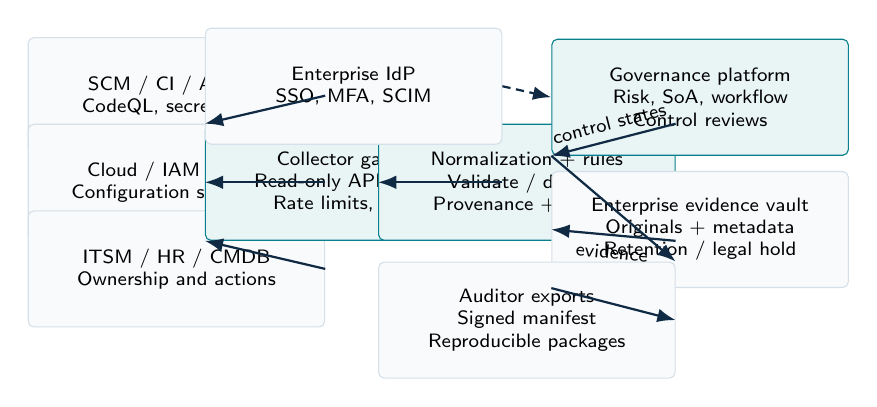
\begin{tikzpicture}[font=\sffamily\scriptsize,nd/.style={draw=line,rounded corners=2pt,fill=paper,align=center,text width=1.39in,minimum height=0.58in},svc/.style={nd,draw=teal,fill=pale},arr/.style={-Latex,thick,draw=navy}]
\node[nd] (scm) at (0,1.6) {SCM / CI / AppSec\\ CodeQL, secret alerts};
\node[nd] (cloud) at (0,0.5) {Cloud / IAM / EDR\\ Configuration snapshots};
\node[nd] (itsm) at (0,-0.6) {ITSM / HR / CMDB\\ Ownership and actions};
\node[svc] (ingest) at (2.25,0.5) {Collector gateway\\ Read-only APIs, queue\\ Rate limits, retries};
\node[svc] (validate) at (4.45,0.5) {Normalization + rules\\ Validate / dedupe\\ Provenance + hashes};
\node[svc] (grc) at (6.65,1.58) {Governance platform\\ Risk, SoA, workflow\\ Control reviews};
\node[nd] (store) at (6.65,-0.1) {Enterprise evidence vault\\ Originals + metadata\\ Retention / legal hold};
\node[nd] (exports) at (4.45,-1.25) {Auditor exports\\ Signed manifest\\ Reproducible packages};
\node[nd] (idp) at (2.25,1.72) {Enterprise IdP\\ SSO, MFA, SCIM};
\draw[arr] (scm.east) -- (ingest.north west);
\draw[arr] (cloud.east) -- (ingest.west);
\draw[arr] (itsm.east) -- (ingest.south west);
\draw[arr] (ingest.east) -- (validate.west);
\draw[arr] (validate.north east) -- node[above,sloped]{control states} (grc.south west);
\draw[arr] (validate.south east) -- node[below,sloped]{evidence} (store.west);
\draw[arr] (store.south west) -- (exports.east);
\draw[arr] (grc.south west) -- (exports.north east);
\draw[arr,densely dashed] (idp.east) -- (grc.west);
\end{tikzpicture}
\caption{Reference pattern: governance system of record plus independently governed evidence pipeline. Dashed: identity federation.}
\end{figure}
\begin{noteBox}
\textbf{System-of-record contract.} The governance platform is authoritative for control owners, applicability, risk decisions, approvals and finding status. Source systems are authoritative for observed security events. The evidence vault is authoritative for original, preserved payloads and signed manifests. The integration service must never silently rewrite an approved risk acceptance or SoA entry.
\end{noteBox}

\subsection{Architecture options: deployment and ownership}

\begin{tabularx}{\linewidth}{@{}L{1.35in}YYY@{}}
\toprule
\textbf{Component} & \textbf{Build B1} & \textbf{Buy P1} & \textbf{Hybrid H1}\\\midrule
Risk / SoA / policy state & Internal database & Vendor product & Vendor product\\
User experience / workflows & Internal UI + rules & Vendor UI & Vendor UI + integration status\\
Control evidence collectors & Internally developed & Supplier integrations & Internally governed collectors\\
Evidence originals & Organization-managed & Supplier storage (verify terms) & Organization vault by default\\
Hosting and DR & Internal platform/SRE & Vendor, contract-backed & Shared by defined boundaries\\
API and data mapping & Internal service & Vendor APIs/config & Internal integration contract\\
Security patching & Internal app owner & Vendor app; buyer config & Shared and explicitly assigned\\
\bottomrule
\end{tabularx}

\subsection{Evidence lifecycle and chain of custody}
\begin{figure}[H]
\centering
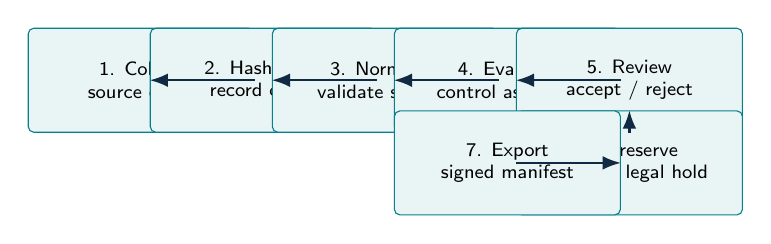
\begin{tikzpicture}[font=\sffamily\scriptsize,phasebox/.style={draw=teal,fill=pale,rounded corners=2pt,minimum width=1.13in,minimum height=0.52in,align=center},arr/.style={-Latex,thick,draw=navy}]
\node[phasebox] (a) at (0,0) {1. Collect\\ source event};
\node[phasebox] (b) at (1.55,0) {2. Hash, date\\ record origin};
\node[phasebox] (c) at (3.10,0) {3. Normalize\\ validate schema};
\node[phasebox] (d) at (4.65,0) {4. Evaluate\\ control assertion};
\node[phasebox] (e) at (6.20,0) {5. Review\\ accept / reject};
\node[phasebox] (f) at (6.20,-1.05) {6. Preserve\\ expiry / legal hold};
\node[phasebox] (g) at (4.65,-1.05) {7. Export\\ signed manifest};
\draw[arr] (a) -- (b);
\draw[arr] (b) -- (c);
\draw[arr] (c) -- (d);
\draw[arr] (d) -- (e);
\draw[arr] (e) -- (f);
\draw[arr] (f) -- (g);
\end{tikzpicture}
\caption{Automated observations and human control conclusions are different records.}
\end{figure}
\textbf{Minimum provenance envelope:} source-system identifier; collector service identity and version; source event ID and effective time; observed/ingested time; scope ID; asset/control references; content checksum; transformation rule and version; reviewer identity and decision; retention label; export-bundle identifier. Record UTC timestamps and timezone offsets in views. Preserve originals where law and contracts permit.

\subsection{Minimal canonical information model}

\begin{tabularx}{\linewidth}{@{}L{1.23in}L{1.65in}Y@{}}
\toprule
\textbf{Entity} & \textbf{Key fields} & \textbf{Integrity condition}\\\midrule
Risk & \texttt{risk\_id}, method version, owner, score & Approved changes and decision history\\
Control & \texttt{control\_id}, framework mapping, owner & One durable implementation ID across mapped frameworks\\
SoA decision & \texttt{soa\_id}, applicability, rationale, approver & Linked to risk assessment and SoA version\\
Evidence & \texttt{evidence\_id}, source, checksum, collected & Immutable original + independently mutable review status\\
Evaluation & \texttt{test\_id}, rule version, result & Reproducible test inputs and human override reason\\
Finding & \texttt{finding\_id}, severity, assignee, due & Distinct from accepted risk and exception record\\
Action & \texttt{action\_id}, action owner, validation & Verify effectiveness after purported remediation\\
Audit event & \texttt{event\_id}, actor, verb, time & Ordered, protected, queryable and exportable\\
\bottomrule
\end{tabularx}

\subsection{Representative API envelope (non-normative)}
\begin{lstlisting}[language={},caption={Illustrative normalized evidence record; not an ISO-prescribed schema.}]
{
  "evidence_id": "ev-01HV...",
  "source": {"system": "github", "resource_id": "org/repo"},
  "scope_id": "isms-prod-us",
  "control_id": "CTRL-APPSEC-004",
  "observed_at": "2026-10-01T14:04:22Z",
  "collected_at": "2026-10-01T14:05:18Z",
  "collector": {"name": "source-adapter", "version": "2.3.1"},
  "payload_sha256": "<64-lowercase-hex-characters>",
  "vault_uri": "evidence://vault/ev-01HV...",
  "classification": "internal-confidential",
  "evaluation": {"rule_version": "7", "result": "review"},
  "review": {"status": "pending", "reviewer_id": null},
  "retention_policy": "ISMS-RECORDS-01"
}
\end{lstlisting}
\textbf{Contract requirements.} Idempotent ingestion key; cursor-based pagination; bounded queues and exponential backoff; replay with de-duplication; data-minimizing payload shapes; versioned schemas; non-repudiable audit events where feasible; revocable source tokens; quarantine of malformed data; and dead-letter monitoring. Never store secrets or full customer payloads where summary metrics suffice.

\subsection{Security and privacy threat model}
\small

\begin{longtable}{@{}L{1.45in}L{2.05in}L{2.78in}@{}}
\toprule
\textbf{Threat} & \textbf{Trust boundary at risk} & \textbf{Recommended mitigation / test}\\\midrule\endhead
Collector token compromise & Internal evidence gateway to source & Read-only, scoped permissions; rotation; workload identity; theft simulation\\
Fabricated ``passing'' evidence & Source API to normalized control state & Source origin, immutable receipt hash, signed provenance, independent sample\\
Over-permissive auditor access & GRC tenant to confidential evidence & Role-scoped exports, timeboxed access, access review\\
Cross-tenant data exposure & SaaS tenant isolation & Vendor testing evidence; tenant boundary review; contractual controls\\
Malicious or faulty integration & Source adapters to governance system & Schema validation, code review, pin versions, isolation and throttling\\
Changed supplier retention & Vendor storage and deletion services & Contractual control, exit drill, data-retention test\\
Obsolete evidence incorrectly trusted & Collection date vs audit period & Freshness threshold; test-period attribution and explicit exception\\
Ransomware / destructive admin & Operational stores and backup plane & Immutable backups, key separation, restore tests\\
Source system outage & Control telemetry freshness & Recorded gaps, retries, incident escalation, alternate manual control\\
Misleading framework mapping & External mapping library to SoA & Version pinning, owner review; no implication of one-to-one equivalence\\
\bottomrule
\end{longtable}
\normalsize

\section{Evaluation methodology and procurement process}
\subsection{Stage-gated lifecycle}
\begin{enumerate}
\item \textbf{Discover}: map ISMS obligations, stakeholder goals, current-state workflows, constraints and baseline costs.
\item \textbf{Qualify}: issue evidence-backed RFI, reject hard-gate failures and record known gaps.
\item \textbf{Demonstrate}: run scripted proof of concept (PoC) in an approved sandbox, using the same dataset for every candidate.
\item \textbf{Score}: perform panel scoring only after the demonstration; record evidence links and dissenting views.
\item \textbf{Price}: normalize contract/licensing structures and internal engineering effort into comparable TCO.
\item \textbf{Decide}: architecture review, security/privacy/legal sign-off, financial approval, and an auditable Architecture Decision Record (ADR).
\item \textbf{Deliver}: phase gates; reassess scope, data flow, assumptions and residual risk at go-live.
\end{enumerate}

\subsection{Comparable PoC scenarios}
\small

\begin{longtable}{@{}L{0.50in}L{3.04in}L{2.80in}@{}}
\toprule
\textbf{Test} & \textbf{Script} & \textbf{Pass evidence}\\\midrule\endhead
P-01 & Create risk, assess it, approve treatment, and create SoA decision & History shows methodology version, owner and rationale\\
P-02 & Ingest code scanning alert with source API ID; dismiss as false match at source & Native/source provenance retained; mapping does not erase source disposition\\
P-03 & Change cloud asset scope; re-evaluate affected control & Coverage gaps surfaced and explicit reassessment initiated\\
P-04 & Delete and restore test evidence via approved procedure & Validated retention, purge limits and recoverability\\
P-05 & Disable employee at IdP; attempt GRC and API access & Access revoked within agreed time; event logged\\
P-06 & Generate audit sample for a historical 60-day period & Correct time range, original documents, review and checksum included\\
P-07 & Create issue and corrective action, test closure & No automatic closure merely because ticket status changed\\
P-08 & Force source API errors and rate limits & Exponential retry, no duplicates, dead-letter and alert visible\\
P-09 & Export all scoped entities and attachments to nonproprietary formats & Independent parser can reconstruct links and review timeline\\
P-10 & Run management review with an overdue risk and unresolved exception & Decision pack accurate; minutes/actions approved and linked\\
\bottomrule
\end{longtable}
\normalsize

\subsection{Weighted multi-criteria decision analysis (MCDA)}
For feasible alternatives, score each criterion from 1 (materially inadequate) to 5 (exceptionally well supported) against a common rubric and evidence, then normalize to 100:
\begin{equation}\label{eq:score}
S_a = \frac{1}{5}\sum_{i=1}^{n} w_i r_{a,i},\quad \sum_i w_i=100,\quad r_{a,i}\in\{1,2,3,4,5\}.
\end{equation}
\textit{Never let this ranking override a non-waivable gate; use interval/range estimates when scoring uncertainty is material.}


\begin{tabularx}{\linewidth}{@{}L{2.31in}R{0.68in}R{0.89in}R{0.89in}R{0.89in}@{}}
\toprule
\textbf{Criterion} & \textbf{Weight \%} & \textbf{Build} & \textbf{Buy} & \textbf{Hybrid}\\\midrule
Time to usable control/audit workflows & 15 & 2 & 5 & 4\\
Functional fit and configurability & 20 & 5 & 4 & 5\\
Integrations and data ownership & 15 & 5 & 3 & 5\\
Security and operational assurance & 15 & 3 & 4 & 4\\
Cost/value (whole-life, not price only) & 15 & 3 & 4 & 4\\
Exit, portability and strategic flexibility & 10 & 5 & 2 & 4\\
Operations and delivery capacity fit & 10 & 2 & 4 & 3\\\midrule
\textbf{Weighted score / 100} & \textbf{100} & \textbf{73} & \textbf{76} & \textbf{85}\\
\bottomrule
\end{tabularx}
\figsource{Illustrative panel judgments, not supplier performance claims. All weights and evidence ratings must be ratified by an evaluation committee.}

\subsection{Scoring rubric and evidence confidence}

\begin{tabularx}{\linewidth}{@{}L{0.5in}L{1.95in}Y@{}}
\toprule
\textbf{Rating} & \textbf{Interpretation} & \textbf{Evidence rule}\\\midrule
1 & Unfit / unproven & No working capability, unacceptable workarounds\\
2 & Substantial gap & Limited demo; large compensating controls or roadmap dependence\\
3 & Meets baseline & Scripted demonstration passes with manageable limitations\\
4 & Strong capability & Repeatable proof, operational metrics, adequate documentation\\
5 & Leading fit & Repeatable proof across edge cases, strong independent evidence\\
\bottomrule
\end{tabularx}
Add confidence \textbf{A = independently tested}, \textbf{B = witnessed sandbox proof}, \textbf{C = documentation or supplier assertion}, \textbf{D = unknown}. Scores rated C or D must have evidence collection plans, and D cannot satisfy a hard gate.

\subsection{Vendor evaluation and RFP scorecard}
\small

\begin{longtable}{@{}L{1.45in}L{2.38in}L{2.50in}@{}}
\toprule
\textbf{Category} & \textbf{Vendor response requested} & \textbf{Buyer verification method}\\\midrule\endhead
Product scope & Supported ISO 27001 workflows, versions, roadmap and exclusions & Run P-01, P-07, P-10\\
Integration & Source systems, API docs, quotas, event semantics, connector ownership & Run P-02, P-03, P-08; inspect API terms\\
Data lifecycle & Processing locations, subprocessors, backups, legal holds, deletion & ROPA/transfer review; P-04, P-09\\
Identity & SSO/SAML/OIDC, MFA, SCIM, admin segregation & P-05 and privileged-admin walkthrough\\
Assurance & Applicable independent attestations, scope, exceptions, incident history & Obtain current reports under NDA; evaluate carve-outs\\
Resilience & SLA, architecture, RTO/RPO, restore testing, status history & Review measured evidence and service commitments\\
Security & Secure development, pentest scope, vulnerability response, encryption & Security due diligence and risk-owner approval\\
Customer operations & Deployment staffing, onboarding, support tier and timelines & References and support escalation exercise\\
Commercial & All subscription units, price escalators, overages, professional services & Five-year normalized quotation and scenario model\\
Exit & Accessible exports, supported migration, deletion certificate, continued access & P-09 with independent parser and dry run\\
Contract terms & Audit rights, liability, notification, IP, subprocessor notices & Legal/procurement exception register\\
\bottomrule
\end{longtable}
\normalsize
\subsection{Procurement deliverables}
Issue a requirements annex with IDs and priorities; supplier response with \textbf{supported / configurable / custom / roadmap / unsupported}; requested proof; standard and data-processing agreements; pricing schedule; service description; interface specifications; evaluation workbook; PoC scripts; risk register; and a proposed transition-out plan. Require suppliers to state which roadmap claims are contractual commitments versus non-binding aspirations.

\section{Five-year total cost of ownership and value model}\label{sec:finance}
\subsection{Financial comparability rules}
Use a single time horizon, salary/contractor loaded rates, audit-period assumptions, currency, inflation method, year-zero date, discount rate, integration count, availability level, data volume, and accounting treatment. Separate \textbf{incremental option-specific costs} from \textbf{common ISMS costs}, such as risk owners, executives, required internal audits and certification fees (if any), which persist regardless of platform. Include common costs in the enterprise budget; exclude them \emph{equally} from comparative TCO if genuinely identical. Do not count a staff-hour saving both as avoided cash expense and productivity benefit without approved monetization.

\subsection{Cost taxonomy}

\begin{tabularx}{\linewidth}{@{}L{1.27in}L{2.65in}Y@{}}
\toprule
\textbf{Category} & \textbf{Included examples} & \textbf{Common exclusion error}\\\midrule
Year-zero investment & Discovery, design, integrations, migration, validation, training & Omitting staff time and review cycles\\
Recurring subscription & Seats, modules, API usage, evidence volume, support tiers & Ignoring minimums, volume steps, renewals\\
Internal operations & Security engineering, SRE, integration support, platform admin & Assuming vendor operation means zero buyer labor\\
Infrastructure & Compute, secrets, storage, logs, backups, bandwidth & Assuming internal software is free to run\\
Assurance & Product review, independent testing, annual reassessment & Treating a compliance dashboard as an audit\\
Migration and exit & Data extraction, mapping, revalidation, dual run and deletion & Modeling supplier cancellation as cost-free\\
Uncertainty & Rate volatility, scope expansion, outage and delivery delay & Hiding risk premium inside score rather than model\\
\bottomrule
\end{tabularx}

\subsection{Formula and financial assumptions}
Let $I_a$ be year-zero implementation, $O_{a,1}$ the first-year operating cost, $g_a$ annual growth, $d$ annual discount rate, and $T$ the number of operating years for alternative $a$. End-of-year cash-flow convention:
\begin{align}
O_{a,t}&=O_{a,1}(1+g_a)^{t-1}, \qquad t=1,\ldots,T,\\
\mathrm{TCO}^{\mathrm{nom}}_a(T)&=I_a+\sum_{t=1}^{T}O_{a,t},\\
\mathrm{NPV\ Cost}_a(T)&=I_a+\sum_{t=1}^{T}\frac{O_{a,t}}{(1+d)^t},\\
\mathrm{Net\ Benefit}_a&=\mathrm{NPV}({\text{incremental validated benefits}})-\mathrm{NPV\ Cost}_a.
\end{align}
For all results below: $T=5$, $d=10\%$, and values are \textbf{USD thousands}. These are nominal assumed cash flows (not accounting capitalizations, forecasts, price commitments or observed market averages). No tax, residual resale value, probabilistic incident loss or audit-fee savings are included.


\begin{tabularx}{\linewidth}{@{}L{2.3in}R{1.15in}R{1.15in}R{1.15in}@{}}
\toprule
\textbf{Assumption, USD \$000} & \textbf{Build B1} & \textbf{Buy P1} & \textbf{Hybrid H1}\\\midrule
Year-zero design / implementation / validation & 260 & 95 & 155\\
Year-one option-specific operating expense & 160 & 150 & 135\\
Annual operating escalation & 4\% & 5\% & 4\%\\
Discount rate & 10\% & 10\% & 10\%\\
Common ISMS program costs & Excluded & Excluded & Excluded\\
\bottomrule
\end{tabularx}

\subsection{Transparent cost decomposition}

\begin{tabularx}{\linewidth}{@{}L{2.15in}R{1.20in}R{1.20in}R{1.20in}@{}}
\toprule
\textbf{Year-zero investment component} & \textbf{Build} & \textbf{Buy} & \textbf{Hybrid}\\\midrule
Discovery and platform configuration/design & 65 & 45 & 45\\
Development, custom automation / major setup & 140 & 0 & 75\\
Data migration and integration & 35 & 30 & 15\\
Training, validation and deployment & 20 & 20 & 20\\\midrule
\textbf{Total year zero} & \textbf{260} & \textbf{95} & \textbf{155}\\
\bottomrule
\end{tabularx}

\begin{tabularx}{\linewidth}{@{}L{2.15in}R{1.20in}R{1.20in}R{1.20in}@{}}
\toprule
\textbf{Year-one operating component} & \textbf{Build} & \textbf{Buy} & \textbf{Hybrid}\\\midrule
Platform engineering / integration support & 138 & 20 & 45\\
Platform software subscription & 0 & 105 & 70\\
Infrastructure, vault and telemetry & 12 & 0 & 10\\
Platform administration and specialized support & 10 & 25 & 10\\\midrule
\textbf{Total year one} & \textbf{160} & \textbf{150} & \textbf{135}\\
\bottomrule
\end{tabularx}
\figsource{All entries are designed to be mutually exclusive within each option. Examples only; change internal rates, software prices, infra, support and work scopes to organization-specific estimates.}

\subsection{Year-by-year model and results}

\begin{tabularx}{\linewidth}{@{}L{1.40in}R{1.45in}R{1.45in}R{1.45in}@{}}
\toprule
\textbf{Cash flow (\$000)} & \textbf{Build} & \textbf{Buy} & \textbf{Hybrid}\\\midrule
Year 0 & 260.00 & 95.00 & 155.00\\
Year 1 & 160.00 & 150.00 & 135.00\\
Year 2 & 166.40 & 157.50 & 140.40\\
Year 3 & 173.06 & 165.38 & 146.02\\
Year 4 & 179.98 & 173.64 & 151.86\\
Year 5 & 187.18 & 182.33 & 157.93\\\midrule
\textbf{Nominal five-year TCO} & \textbf{1,126.61} & \textbf{923.84} & \textbf{886.20}\\
\textbf{Five-year NPV at 10\%} & \textbf{912.14} & \textbf{717.59} & \textbf{705.25}\\
\bottomrule
\end{tabularx}
\begin{figure}[H]
\centering
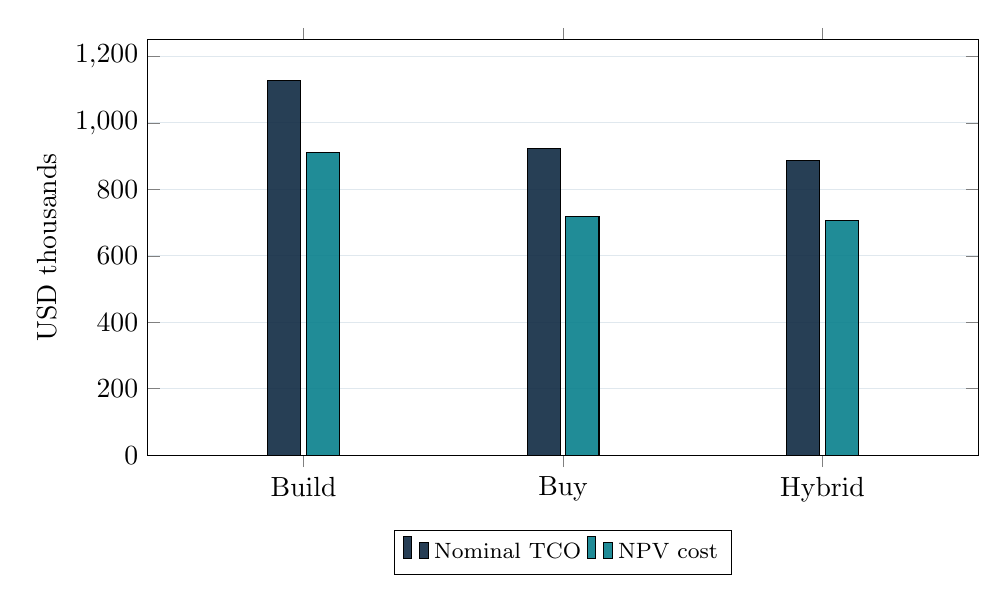
\begin{tikzpicture}
\begin{axis}[width=\linewidth,height=2.7in,ybar,bar width=12pt,ymin=0,ymax=1250,symbolic x coords={Build,Buy,Hybrid},xtick=data,ymajorgrids=true,grid style={line!75},ylabel={USD thousands},legend style={at={(0.5,-0.18)},anchor=north,legend columns=2,font=\footnotesize},every axis plot/.append style={fill opacity=0.9},enlarge x limits=0.3]
\addplot[fill=navy] coordinates {(Build,1126.61) (Buy,923.84) (Hybrid,886.20)};
\addplot[fill=teal] coordinates {(Build,912.14) (Buy,717.59) (Hybrid,705.25)};
\legend{Nominal TCO,NPV cost}
\end{axis}
\end{tikzpicture}
\caption{Five-year illustrative life-cycle cost comparison; lower is preferable, assuming comparable benefit and gate compliance.}
\end{figure}

\subsection{Cumulative break-even and crossover}
For alternatives with constant annual differences, the simplified nominal break-even approximation is:
\[\frac{I_H-I_P}{O_{P,1}-O_{H,1}}=\frac{155-95}{150-135}=4\text{ years}.\]
\textbf{Do not use this approximation for the actual escalated cash flows.} Buy remains nominally cheaper through Year 3, while hybrid becomes cheaper in \textbf{Year 4}. Discounted cumulative costs cross over in \textbf{Year 5} under the assumed 10\% discount rate.

\begin{tabularx}{\linewidth}{@{}L{1.55in}R{1.25in}R{1.25in}R{1.25in}@{}}
\toprule
\textbf{Cumulative cost (\$000)} & \textbf{Build} & \textbf{Buy} & \textbf{Hybrid}\\\midrule
Through Year 0 & 260.00 & 95.00 & 155.00\\
Through Year 1 & 420.00 & 245.00 & 290.00\\
Through Year 2 & 586.40 & 402.50 & 430.40\\
Through Year 3 & 759.46 & 567.88 & 576.42\\
Through Year 4 & 939.43 & 741.52 & \textbf{728.27}\\
Through Year 5 & 1,126.61 & 923.84 & \textbf{886.20}\\
\bottomrule
\end{tabularx}

\subsection{Cost sensitivities and scenario risk}

\begin{tabularx}{\linewidth}{@{}L{2.75in}R{1.25in}R{1.25in}@{}}
\toprule
\textbf{One-factor scenario vs baseline} & \textbf{$\Delta$ 5y nominal (\$000)} & \textbf{$\Delta$ NPV (\$000)}\\\midrule
Buy subscription line +25\%, same escalation & +145.05 & +108.95\\
Build engineering labor line +35\%, same escalation & +261.61 & +196.87\\
Hybrid subscription line +25\%, same escalation & +94.79 & +71.33\\
\bottomrule
\end{tabularx}
\textbf{Scenario interpretation:} Higher buy licensing could widen the gap; higher hybrid licensing could make buy less expensive on a discounted basis. These single-factor cases are \emph{not} probability-weighted expected values and must not be summed unless the joint scenario is intentional.

\textbf{Required finance extensions:} Assess 3/5/7-year horizons; 6/10/14\% discount rates; costs of a delayed launch; seat/evidence volume tiers; termination fees; integration count; exit migration; staff turnover and contractor pricing; product downtime; and contract renewal cliffs. Price incidents as explicit expected-loss scenarios only when validated by enterprise risk/finance, not as arbitrary savings.

\subsection{Benefits ledger and ROI limitations}

\begin{tabularx}{\linewidth}{@{}L{1.45in}L{2.47in}Y@{}}
\toprule
\textbf{Benefit} & \textbf{Operational quantity} & \textbf{Monetization and guardrail}\\\midrule
Reduced evidence collection time & Hours of manual collection avoided per audit cycle & Loaded labor only if released for measurable productive work or reduced spend\\
Faster control gap discovery & Median days from failing condition to owner notice & Avoided-loss attribution requires separate probabilistic method\\
Lower audit coordination & Auditor questions, rework hours and missing artifacts & Do not assume reduction without historical baseline\\
Better management visibility & Decision latency, approved overdue risks & Usually a qualitative benefit; avoid fabricated dollar values\\
Improved portability & Verified export/recovery time and exit cost & Model through exit scenario rather than duplicate ROI line\\
\bottomrule
\end{tabularx}

\section{Risk register and mitigations}
\small

\begin{longtable}{@{}L{0.58in}L{1.76in}L{1.98in}L{1.86in}@{}}
\toprule
\textbf{ID} & \textbf{Risk and cause} & \textbf{Exposure / early signal} & \textbf{Owner / treatment}\\\midrule\endhead
R-01 & Supplier lock-in, poor export & Proprietary IDs, incomplete attachments & Architecture owner: contract + export test\\
R-02 & Evidence cannot be trusted & Missing source, test period or review chain & GRC lead: provenance controls + sampling\\
R-03 & Shadow ISMS records & Risk or SoA data in overlapping apps & ISMS owner: nominate data authority\\
R-04 & Privacy or residency breach & Unapproved SaaS ingestion of sensitive files & Privacy lead: classify/minimize/approve flows\\
R-05 & Internal product under-resourced & Bus factor, backlog and incident delays & CTO: funded staffing, SLO and succession\\
R-06 & Vendor material service outage & Missed reviews or inaccessible audit packets & Vendor manager: resilience and offline exports\\
R-07 & Inaccurate control mapping & Auto-passing results with no applicability context & Control owner: manual approval and QA\\
R-08 & Unbudgeted consumption & Seats/API/evidence tiers rise unexpectedly & Finance: usage caps, forecast and sensitivity\\
R-09 & Control fatigue and noisy findings & Alert volumes overwhelm reviewers & GRC lead: prioritization, quality metrics\\
R-10 & Framework/version drift & Mapping or policy templates become outdated & Compliance owner: controlled change review\\
R-11 & Procurement deadline optimism & Vendor onboarding and security review slip & PMO: critical path and contingencies\\
R-12 & Misstated independence & Owners certify their own audit conclusions & Internal audit: role separation\\
\bottomrule
\end{longtable}
\normalsize
Rate each risk using the organization's approved likelihood/impact method; assign a treatment and deadline; capture decision authority and residual acceptance. This template intentionally does not invent numerical risk ratings.

\section{Implementation strategy, work breakdown and delivery gates}
\subsection{Prerequisite-oriented roadmap}

\begin{tabularx}{\linewidth}{@{}L{1.13in}L{1.36in}L{2.35in}Y@{}}
\toprule
\textbf{Phase} & \textbf{Indicative weeks} & \textbf{Deliverables} & \textbf{Exit gate}\\\midrule
0. Mobilize & 0--2 & Sponsor, project charter, scope, baseline systems and risks & Decision owners named; initial budget and audit targets\\
1. Baseline & 2--5 & ISO requirement mapping, ISMS process maps, gap and data-classification inventory & Validated scope; current-state and requirements approval\\
2. Market/architecture & 5--9 & RFI/RFP, B1/P1/H1 alternatives, vendor shortlist, architecture/data flows & All candidates assessed against hard gates\\
3. PoC and decision & 9--13 & Scripted demonstrations, risk review, TCO, MCDA, signed ADR & Selection rationale, security/legal/finance approval\\
4. Foundation & 13--17 & Tenant/environment, IAM, control taxonomy, data model, audit log & Foundational NFR evidence and operating ownership\\
5. Integrations & 17--22 & Priority sources, evidence vault, testing, review workflow, pilot scope & E2E evidence trace and exception/retry demonstration\\
6. Readiness & 22--26 & Training, runbooks, management review, audit simulation, DR/exit rehearsal & Signed acceptance and go-live decision\\
7. Operate/improve & From 26 onward & KPI cadence, supplier review, audit findings, enhancement backlog & Operating performance evidenced and corrective actions tracked\\
\bottomrule
\end{tabularx}
\figsource{Indicative sequencing only; workstreams overlap. Certification timing depends on actual ISMS maturity, operating evidence and audit arrangements---not this software deployment schedule.}

\subsection{Dependency graph (critical path)}
\begin{figure}[H]
\centering
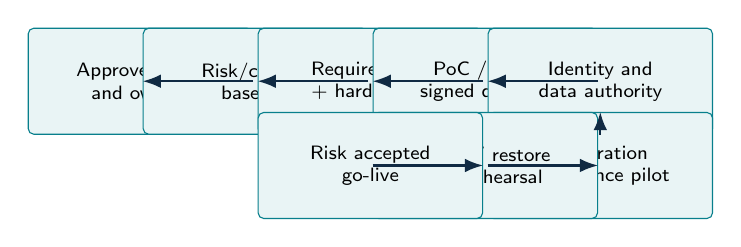
\begin{tikzpicture}[font=\sffamily\scriptsize,phasebox/.style={draw=teal,fill=pale,rounded corners=2pt,align=center,text width=1.03in,minimum height=0.53in},arr/.style={-Latex,thick,draw=navy}]
\node[phasebox] (a) at (0,0) {Approve scope\\ and owners};
\node[phasebox] (b) at (1.46,0) {Risk/control\\ baseline};
\node[phasebox] (c) at (2.92,0) {Requirements\\ + hard gates};
\node[phasebox] (d) at (4.38,0) {PoC / TCO\\ signed decision};
\node[phasebox] (e) at (5.84,0) {Identity and\\ data authority};
\node[phasebox] (f) at (5.84,-1.07) {Integration\\ + evidence pilot};
\node[phasebox] (g) at (4.38,-1.07) {Audit / restore\\ exit rehearsal};
\node[phasebox] (h) at (2.92,-1.07) {Risk accepted\\ go-live};
\foreach \x/\y in {a/b,b/c,c/d,d/e,e/f,f/g,g/h}{\draw[arr] (\x) -- (\y);}
\end{tikzpicture}
\caption{Dependencies emphasize risk scope and data governance before connector deployment.}
\end{figure}

\subsection{RACI (recommended owner model)}

\begin{tabularx}{\linewidth}{@{}L{2.51in}L{0.61in}L{0.61in}L{0.61in}L{0.61in}L{0.61in}@{}}
\toprule
\textbf{Activity} & \textbf{CISO} & \textbf{GRC} & \textbf{Arch.} & \textbf{Eng.} & \textbf{Audit}\\\midrule
Scope and risk policy & A & R & C & I & C\\
Requirement specification & A & R & R & C & C\\
Architecture and data flows & C & C & A & R & I\\
Vendor security due diligence & A & R & C & C & C\\
Integration and secure deployment & I & C & A & R & I\\
Evidence ownership and quality & A & R & C & R & C\\
Independent internal-audit conclusion & I & C & I & I & A/R\\
Management review and risk decision & A & R & C & I & C\\
\bottomrule
\end{tabularx}
\figsource{Example only. R=responsible, A=accountable, C=consulted, I=informed. Finance, procurement, privacy and legal are mandatory contributors for their respective decisions even where omitted from this compact matrix.}

\subsection{Acceptance criteria and release readiness}
\begin{enumerate}
\item 100\% of \textbf{M} requirements have passing scripted tests or explicitly approved, time-bounded exceptions with accountable residual risk.
\item Each production connector demonstrates input validation, token scoping, replay/idempotency, failure monitoring, reconciliation and owner handover.
\item All pilot risks and controls have accountable owners, SoA links, defined evidence cadence and explicit current/overdue status.
\item An auditor can independently navigate a sampled evidence path and reconstruct a historical status without privileged engineering intervention.
\item Backup restore and exit export are tested to the approved recovery and portability objectives.
\item The service support matrix, security response, vendor escalation, runbooks, records schedule and management reporting are approved.
\item No critical unaccepted security or privacy risks remain; operational exceptions have review dates and compensating controls.
\end{enumerate}

\section{Continuous assurance and operating measurements}
\subsection{Service-level objectives and value evidence}
\small

\begin{longtable}{@{}L{1.61in}L{2.48in}L{2.00in}@{}}
\toprule
\textbf{Metric} & \textbf{Definition} & \textbf{Owner / cadence}\\\midrule\endhead
Scoped control ownership & $\frac{\text{in-scope controls with active owner}}{\text{total in-scope controls}}\times100\%$ & GRC / weekly\\
Evidence freshness & $\frac{\text{applicable evidence objects within age SLO}}{\text{total applicable evidence objects}}\times100\%$ & Platform ops / daily\\
Automated evidence coverage & $\frac{\text{controls with validated automation}}{\text{controls eligible for automation}}\times100\%$ & Engineering / monthly\\
Collector success rate & $\frac{\text{successful scheduled runs}}{\text{all completed scheduled runs}}\times100\%$ & SRE / daily\\
Overdue actions & Count after due date, split by severity, business owner and days overdue & Risk owner / weekly\\
Evidence rejection rate & $\frac{\text{rejected evidence reviews}}{\text{all completed evidence reviews}}\times100\%$ & GRC / monthly\\
Risk acceptance freshness & Share of approvals reviewed by or before their next-review dates & CISO delegate / monthly\\
Restore success & Successful restore rehearsals / planned rehearsal count & SRE + security / quarterly\\
Audit evidence latency & Median hours from sampled request to verified auditor packet & Audit liaison / audit cycle\\
Manual effort avoided & Baseline hours minus measured steady-state hours, like-for-like & Finance + GRC / quarterly\\
\bottomrule
\end{longtable}
\normalsize
\textbf{Measurement safeguards:} Define eligibility, lookback, exclusions, evidence sampling, population source, collection errors and metric owner. A near-100\% automated-evidence rate is not synonymous with complete risk coverage, control effectiveness, or ISO conformity. Establish baselines in pilot before setting improvement targets.

\subsection{Operational cadence}

\begin{tabularx}{\linewidth}{@{}L{0.95in}Y@{}}
\toprule
\textbf{Cadence} & \textbf{Representative activities}\\\midrule
Daily & Connector availability, new failures, secret/token health, high-risk drift alerts\\
Weekly & Risk/action backlog, evidence exceptions, access/deprovisioning quality, ingestion lag\\
Monthly & Control owner reviews, selected evidence sampling, cost and consumption variance, supplier incident trends\\
Quarterly & Management review inputs, vendor assurance changes, restores, risk reassessment triggers, roadmap reprioritization\\
Annual / triggered & Internal audit program, policy and SoA review, supplier renewal and exit tests, material-change assessment\\
\bottomrule
\end{tabularx}

\section{Decision record, contract checklist and reuse templates}
\subsection{Architecture Decision Record --- fillable template}
\begin{noteBox}
\textbf{ADR-ISMS-001 \quad Status:} Proposed / Accepted / Rejected / Superseded\par
\textbf{Decision date / sponsor / approver:} \rule{3.2in}{0.4pt}\par
\textbf{Business objectives and deadline:} \rule{3.2in}{0.4pt}\par
\textbf{Scope, exclusions, regulated data:} \rule{3.35in}{0.4pt}\par
\textbf{Options and non-negotiable gates:} \rule{3.05in}{0.4pt}\par
\textbf{PoC evidence and confidence:} \rule{3.3in}{0.4pt}\par
\textbf{Five-year NPV / sensitivity / cost owner:} \rule{2.5in}{0.4pt}\par
\textbf{Selected option and rationale:} \rule{3.38in}{0.4pt}\par
\textbf{Risks accepted, mitigations and due dates:} \rule{2.4in}{0.4pt}\par
\textbf{Supersession trigger and review date:} \rule{2.75in}{0.4pt}
\end{noteBox}

\subsection{Contract and exit redlines}
\begin{enumerate}
\item \textbf{Scope and charges:} Precise license units, API limits, attachments, price increases, overages and renewal notice periods.
\item \textbf{Data control:} Controller/processor roles where applicable, allowed purposes, subprocessors, regions, retention, backup, legal hold and cross-border mechanisms.
\item \textbf{Security:} SSO, incident notification periods, evidence of assurance, customer notification for material control changes, vulnerability remediation, administrator access safeguards.
\item \textbf{Availability:} Uptime definition, exclusions, RPO/RTO, support escalation, chronic failure remedy and disaster recovery exercises.
\item \textbf{Portability:} Export endpoint, native originals, machine-readable object relationships, stable identifiers, audit events, historical approvals and documented schema.
\item \textbf{Exit:} Transition support, limited post-termination retrieval window, deletion certificate, remaining backups and subcontractor obligations.
\item \textbf{Governance:} Audit rights proportionate to confidentiality, right to review current assurance, breach handling, subcontractor change notices, IP and data ownership.
\end{enumerate}

\subsection{Decision triggers for revisiting a deployed option}
Reassess after: framework revision; new geographic or regulated-data scope; major incident; failed export/restore exercise; material vendor acquisition or outage; more than one year of unplanned cost escalation; growth beyond API/storage limits; unsupported critical integration; persistent unmet evidence SLO; or unacceptable labor/recruitment dependency.

\subsection{Practical starting configurations}
\textbf{Small, straightforward program:} Favor fit-for-purpose buy if configuration, export and privacy gates pass; limit custom code. \textbf{Large regulated enterprise:} Favor assessed hybrid if source telemetry is heterogeneous and internal security integration engineering is funded. \textbf{Specialized/offline environment:} Consider build or self-hosted commercial option with documented full-lifecycle ownership and evidence of auditor interoperability. These are \emph{hypotheses}, not automatic procurement decisions.

\section{Reference bibliography and verification notes}
\begin{thebibliography}{99}\small
\bibitem{iso27001} ISO/IEC 27001:2022, \emph{Information security, cybersecurity and privacy protection---Information security management systems---Requirements}. ISO, October 2022. \url{https://www.iso.org/standard/27001}.
\bibitem{iso27001am} ISO/IEC 27001:2022/Amd 1:2024, \emph{Amendment 1: Climate action changes}. ISO, February 2024. \url{https://www.iso.org/standard/88435.html}.
\bibitem{iso27002} ISO/IEC 27002:2022, \emph{Information security controls}. ISO, February 2022. \url{https://www.iso.org/standard/75652.html}.
\bibitem{iso27005} ISO/IEC 27005:2022, \emph{Guidance on managing information security risks}. ISO, October 2022. \url{https://www.iso.org/standard/80585.html}.
\bibitem{iso19011} ISO 19011:2026, \emph{Guidelines for auditing management systems}. ISO, May 2026. \url{https://www.iso.org/standard/19011}.
\bibitem{nistcsf} NIST, \emph{The NIST Cybersecurity Framework (CSF) 2.0}, CSWP 29, February 2024. \url{https://doi.org/10.6028/NIST.CSWP.29}.
\bibitem{nist161} NIST, \emph{Cybersecurity Supply Chain Risk Management Practices for Systems and Organizations}, SP 800-161 Rev. 1, including November 2024 update. \url{https://csrc.nist.gov/pubs/sp/800/161/r1/upd1/final}.
\bibitem{nist1326} NIST, \emph{Cybersecurity Supply Chain Risk Management: Due Diligence Assessment Quick-Start Guide}, SP 1326, July 2026. \url{https://doi.org/10.6028/NIST.SP.1326}.
\end{thebibliography}
\begin{cautionBox}
\textbf{Primary-source and licensing limitation.} This is an independently authored decision-support document; it paraphrases standard topics and does not reproduce complete normative clauses, copyrighted control texts, or vendor contract conditions. Official ISO catalog pages and NIST publications were checked against their public descriptions in October 2026. Readers require access to the licensed ISO standards for detailed conformity assessment. Financial results and ratings are examples, not observed prices or security performance.
\end{cautionBox}

\appendix
\section{Reusable vendor response form}

\begin{longtable}{@{}L{0.65in}L{2.45in}L{1.44in}L{1.71in}@{}}
\toprule
\textbf{Req ID} & \textbf{Claim and limitation} & \textbf{Proof reference} & \textbf{Evaluator finding}\\\midrule\endhead
FR-03 & \rule{2.05in}{0.4pt} & \rule{1.20in}{0.4pt} & \rule{1.46in}{0.4pt}\\[1pt]
FR-05 & \rule{2.05in}{0.4pt} & \rule{1.20in}{0.4pt} & \rule{1.46in}{0.4pt}\\[1pt]
FR-07 & \rule{2.05in}{0.4pt} & \rule{1.20in}{0.4pt} & \rule{1.46in}{0.4pt}\\[1pt]
FR-10 & \rule{2.05in}{0.4pt} & \rule{1.20in}{0.4pt} & \rule{1.46in}{0.4pt}\\[1pt]
FR-14 & \rule{2.05in}{0.4pt} & \rule{1.20in}{0.4pt} & \rule{1.46in}{0.4pt}\\[1pt]
NFR-02 & \rule{2.05in}{0.4pt} & \rule{1.20in}{0.4pt} & \rule{1.46in}{0.4pt}\\[1pt]
NFR-06 & \rule{2.05in}{0.4pt} & \rule{1.20in}{0.4pt} & \rule{1.46in}{0.4pt}\\[1pt]
NFR-07 & \rule{2.05in}{0.4pt} & \rule{1.20in}{0.4pt} & \rule{1.46in}{0.4pt}\\[1pt]
\bottomrule
\end{longtable}
\textbf{Instructions:} Duplicate rows for the full requirements catalog; cite concrete demo sessions, logs, written commitments, contracts and security findings. Require each response to state \emph{supported / configurable / custom / roadmap / unsupported}, version, license tier, and priced implementation effort.

\section{Reusable financial assumptions and sensitivity worksheet}

\begin{tabularx}{\linewidth}{@{}L{2.45in}YYY@{}}
\toprule
\textbf{Input} & \textbf{Build} & \textbf{Buy} & \textbf{Hybrid}\\\midrule
Implementation and migration & \rule{0.85in}{0.4pt} & \rule{0.85in}{0.4pt} & \rule{0.85in}{0.4pt}\\[1pt]
Year 1 subscriptions and support & \rule{0.85in}{0.4pt} & \rule{0.85in}{0.4pt} & \rule{0.85in}{0.4pt}\\[1pt]
Year 1 internal loaded FTE & \rule{0.85in}{0.4pt} & \rule{0.85in}{0.4pt} & \rule{0.85in}{0.4pt}\\[1pt]
Year 1 infra / vault / log & \rule{0.85in}{0.4pt} & \rule{0.85in}{0.4pt} & \rule{0.85in}{0.4pt}\\[1pt]
Annual escalation & \rule{0.85in}{0.4pt} & \rule{0.85in}{0.4pt} & \rule{0.85in}{0.4pt}\\[1pt]
Migration/exit scenario & \rule{0.85in}{0.4pt} & \rule{0.85in}{0.4pt} & \rule{0.85in}{0.4pt}\\[1pt]
Risk reserve (not double counted) & \rule{0.85in}{0.4pt} & \rule{0.85in}{0.4pt} & \rule{0.85in}{0.4pt}\\[1pt]
\bottomrule
\end{tabularx}
\textbf{Uncertainty distribution:} Record owner, estimate basis, optimistic / central / pessimistic values, and whether cost is committed, variable or avoidable. Recalculate \cref{eq:score} independently of TCO to prevent double counting cost if it is already a scored category.

\section{Implementation deliverables checklist}
\begin{multicols}{2}
\footnotesize
\begin{itemize}[itemsep=1pt,parsep=0pt,leftmargin=1.40em]
\item[$\square$] Approved scope, context, risk appetite, process maps and named sponsors.
\item[$\square$] Stakeholder/obligation register, SoA method and treatment workflow defined.
\item[$\square$] Selected platform architecture with trust boundaries and data flow approvals.
\item[$\square$] Requirements catalog, vendor responses, hard-gate review and PoC outcomes.
\item[$\square$] Normalized five-year TCO, sensitivities, finance approval and ADR.
\item[$\square$] Contracts, data processing, security, incident and exit terms completed.
\item[$\square$] Ownership matrix, roles, SSO/MFA, service identities and retention classes.
\item[$\square$] Original evidence preservation, signed manifest and restore drills validated.
\item[$\square$] Risk register, control mapping, SoA, findings and audits piloted.
\item[$\square$] Training, operational metrics, periodic reviews and continual improvement.
\end{itemize}
\end{multicols}
\normalsize

\begin{center}
\color{teal}\rule{0.62\linewidth}{1pt}\\[1pt]
\sffamily\small\color{muted} END OF REFERENCE FRAMEWORK \quad\textbullet\quad REVIEW BEFORE USE IN A LIVE PROCUREMENT
\end{center}
\end{document}
